% !TEX encoding = UTF-8 Unicode
\documentclass{beamer}

\usepackage{color}
\usepackage{url}
\usepackage[T2A]{fontenc}
\usepackage[utf8]{inputenc}
\usepackage{graphicx}
\usepackage[english,serbian]{babel}
\usepackage{chemfig}
\usepackage[version=3]{mhchem}
\usepackage{multicol}


\mode<presentation>
{
  \usetheme{Warsaw}       
  \usecolortheme{default} 
  \usefonttheme{serif}    
  \setbeamertemplate{navigation symbols}{}
  \setbeamertemplate{caption}[numbered]
} 


\definecolor{mygreen}{rgb}{0,0.6,0}
\definecolor{mygray}{rgb}{0.5,0.5,0.5}
\definecolor{mymauve}{rgb}{0.58,0,0.82}

\usepackage{listings}
\lstset{ 
  backgroundcolor=\color{white},
  basicstyle=\scriptsize\ttfamily,
  breakatwhitespace=false,
  breaklines=true,
  captionpos=b,
  commentstyle=\color{mygreen},
  deletekeywords={...},            
  escapeinside={\%*}{*)},          
  extendedchars=true,
  firstnumber=1,              
  frame=single,	                
  keepspaces=true,
  keywordstyle=\color{blue},     
  language=Python,                
  morekeywords={*,...},
  numbers=left, 
  numbersep=4pt,                  
  numberstyle=\tiny\color{mygray}, 
  rulecolor=\color{black},
  showspaces=false,
  showstringspaces=false,
  showtabs=false,
  stepnumber=1, 
  stringstyle=\color{mymauve},
  tabsize=1,
  title=\lstname
}
\usepackage{pgfpages}
\pgfpagesuselayout{resize to}[%
  physical paper width=8in, physical paper height=6in]

\title{Obrada spam mail-ova metodom klasifikacije }
\author{Tijana Todorov}
\date{\today}

\begin{document}
\begin{frame}
  \titlepage
\end{frame}

\begin{frame}{Pregled}
  \tableofcontents
\end{frame}

\section{Uvod}
\begin{frame}{Uvod}
\begin{itemize}
 \item Spam poruke su zapravo neželjena pošta koja primaocu samo zatrpava sanduče 
 \item Ona može biti nešto što primaoca ne zanima (reklama, online prodavnica...)
 \item Mogu predstavljati opasnost za primaoca ukoliko su zaražene virusom
 \item Cilj je napraviti dobar spam filter koji će odvajati očekivane i neočekivane poruke
\end{itemize}
\end{frame}

\section{Upoznavanje sa podacima}
\subsection*{Upoznavanje sa podacima}
\begin{frame}[fragile]
\frametitle{Upoznavanje sa podacima}
\begin{itemize}
 \item Podaci se nalaze na  \url{https://web.stanford.edu/~hastie/CASI_files/DATA/SPAM.html} pod nazivom \textbf{SPAM.csv}
 \item 4601 email - 1813 prijavljenih spam poruka
 \item 59 atributa
 	\begin{itemize}
 	\item 57 numeričkih - najčešće korišćene reči 
 	\item 2 kategorička binarna atributa - \textbf{spam} i \textbf{testid}  	
 	\end{itemize}
 \item nema null podataka
\end{itemize}
\end{frame}

\subsection*{Podaci}
\begin{frame}[fragile]
\frametitle{Podaci}
\begin{itemize}
    \item \textbf{spam} - označava da li je pošta neželjena ili ne
    \item \textbf{testid} - označava da li se instanca nalazi u trening ili test skupu
    \item 48 atributa - procenat pojavljivanja reči
\textbf{100*broj\_pojavljivanja\_reči / ukupan\_broj\_reči}
	\item 6 atributa (ch; , ch( , ch[ , ch! , ch\$ , ch\#) - procenat pojavljivanja karaktera
\textbf{ 100*broj\_pojavljivanja\_karaktera / ukupan\_broj\_karaktera}
	\item crl.ave - označava prosečnu dužinu neprekidnih nizova velikih slova.
	\item crl.long - označava dužinu najduže sekvence velikih slova.
	\item crl.tot - ukupan broj velikih slova u email poruci.   
\end{itemize}.

\end{frame}

\section{Obrada podataka}
\subsection*{Obrada podataka - SPSS}
\begin{frame}[fragile]
\frametitle{Obrada podataka - SPSS}

\begin{itemize}
 \item Razlika u opsezima podataka
 	\begin{itemize}
 	\item crl.tot - [1 - 15841]
 	\item make - [0 - 4.54]
 	\end{itemize}
 \item Izabrani neki atributi iz celog skupa (all, remove, internet, mail, addresses, business, money)
 \item Vrši se normalizacija pomoću čvora \textbf{\_Norm}
\end{itemize}
\end{frame}

\subsection*{Obrada podataka - Python}
\begin{frame}[fragile]
\frametitle{Obrada podataka - Python}
\begin{lstlisting}
booleandf = df.select_dtypes(include=[bool])
booleanDictionary = {True: "tacno", False: "netacno"}
for column in booleandf:
    df[column] = df[column].map(booleanDictionary)

features1 = df.columns[0]
features5 = df.columns[4]
features9 = df.columns[8]
features10 = df.columns[9]
features12 = df.columns[11]
features16 = df.columns[15]
features17 = df.columns[16]
features19 = df.columns[18]
features26 = df.columns[25]
features = [features5, features9, features10, features12, features16, features17, features19, features26]
x_original = df[features]
x=pd.DataFrame(prep.MinMaxScaler().fit_transform(x_original))
\end{lstlisting}
\end{frame}

\section{Primenjeni algoritmi}
\begin{frame}{Primenjeni algoritmi}
\begin{itemize}
	\item Drveta odlučivanja (SPSS, Python)
	\item Najbliži susedi - KNN (SPSS, Python)
	\item Neuronske mreže (SPSS, Python)
	\item Metod potpornih vektora - SVM (SPSS)
	\item Gausova klasifikacija (Python)
\end{itemize}
\end{frame}


\subsection{Drveta odlučivanja}
\subsubsection*{C5.0 i C\&Rt - SPSS}
\begin{frame}[fragile]
\frametitle{C5.0 i C\&Rt}
\begin{itemize}
 \item Model se pravi pomoću čvora C5.0
 \item Model se pravi pomoću čvora C\&Rt
\end{itemize}
\begin{figure}
\begin{center}
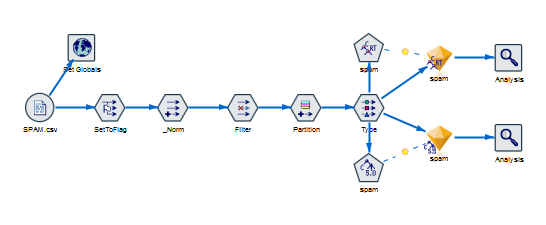
\includegraphics[scale=0.7]{C5CRt_SPSS.png}
\end{center}
\caption{C5.0 i C\&Rt u  SPSS-u}
\end{figure}
\end{frame}

\subsubsection*{C5.0 - SPSS}
\begin{frame}[fragile]
\frametitle{C5.0}
\begin{figure}
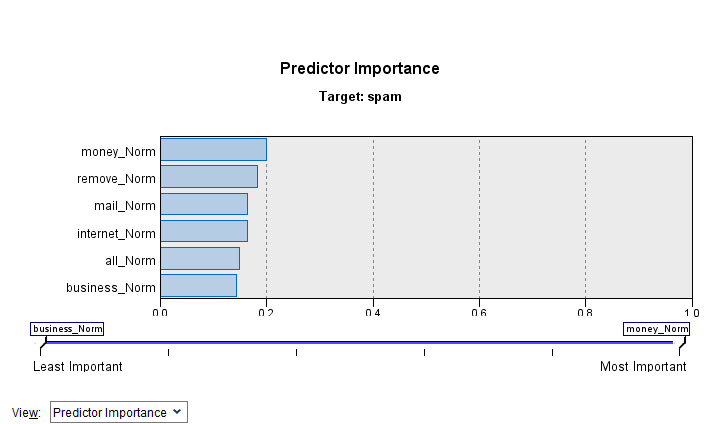
\includegraphics[scale=0.3]{C5_grafik.png}
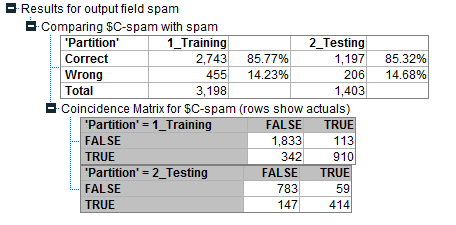
\includegraphics[scale=0.4]{C5Tabela.png}
\caption{Rezultati C5.0 algoritma dobijeni Analyse čvorom u SPSS-u}
\end{figure}
\end{frame}

\subsubsection*{C\&Rt - SPSS}
\begin{frame}[fragile]
\frametitle{C\&Rt}
Drvo dobijeno primenom modela C\&Rt sa sledećim karakteristikama: 
\begin{itemize}
 \item Dubina 3
 \item Broj instanci roditelja 4\% a deteta 2\%
 \item Mera nečistoće - Gini, 0.0001\% 
\end{itemize} 
\begin{figure}
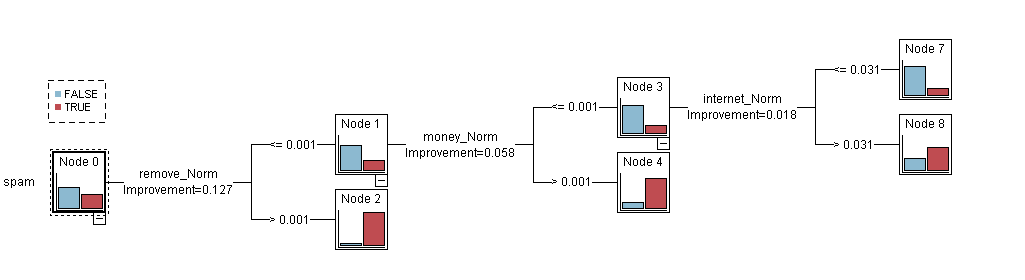
\includegraphics[scale=0.3]{CRtStablo.png}
\caption{Stablo dobijeno C\&Rt algoritmom u SPSS-u}
\end{figure}
\end{frame}

\subsubsection*{C\&Rt - SPSS}
\begin{frame}[fragile]
\frametitle{C\&Rt}
\begin{figure}
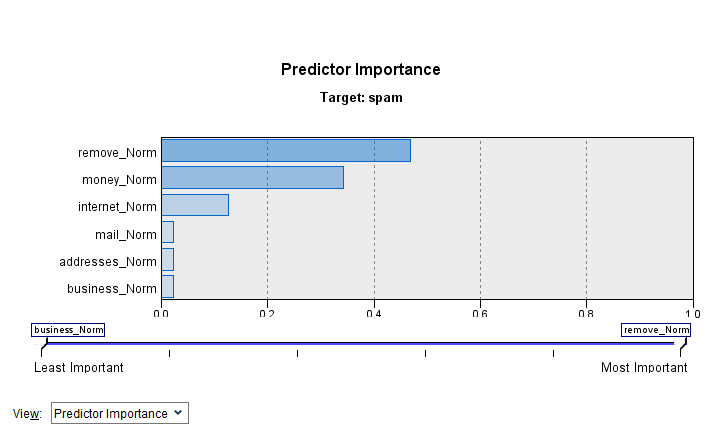
\includegraphics[scale=0.3]{CRtGrafik3.png}
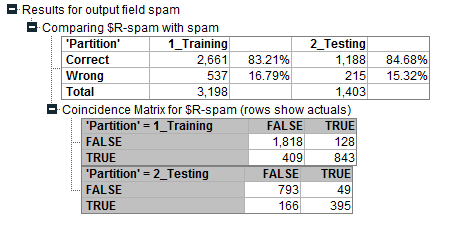
\includegraphics[scale=0.4]{CRtTabela3.png}
\caption{Rezultati C\&Rt algoritma dobijeni Analyse čvorom u SPSS-u}
\end{figure}
\end{frame}

\subsubsection*{Drveta odlučivanja - Python}
\begin{frame}[fragile]
\frametitle{Drveta odlučivanja - Python matrice konfuzije}
\begin{lstlisting}
#Skup  Trening
#Matrica konfuzije
         netacno  tacno
netacno     1882     69
tacno        374    895

Preciznost 0.8624223602484472

#Skup  Test
#Matrica konfuzije
         netacno  tacno
netacno      802     35
tacno        161    383

Preciznost 0.8580738595220855
\end{lstlisting}
\end{frame}

\subsubsection*{Drveta odlučivanja - Python}
\begin{frame}[fragile]
\frametitle{Drveta odlučivanja - Python izveštaji klasifikacije}
\begin{lstlisting}
#Skup Trening
#Izvestaj klasifikacije
              precision    recall  f1-score   support
     netacno       0.83      0.96      0.89      1951
       tacno       0.93      0.71      0.80      1269

#Skup Test
#Izvestaj klasifikacije
              precision    recall  f1-score   support
     netacno       0.83      0.96      0.89       837
       tacno       0.92      0.70      0.80       544

\end{lstlisting}
\end{frame}

\subsection{Najbliži susedi - KNN}
\subsubsection*{Najbliži susedi KNN - SPSS}
\begin{frame}[fragile]
\frametitle{Najbliži susedi - KNN}
\begin{itemize}
\item Sređene podatke povezujemo sa \textit{Partition} čvorom i generišemo model pokretanjem čvora \textit{KNN}.
\item Ciljni atribut je \textit{spam}
\item Minimalni broj k je 3 a maksimalan 5
\item Udaljenost se računa Euklidskim rastojanjem
\end{itemize}
\begin{figure}
\begin{center}
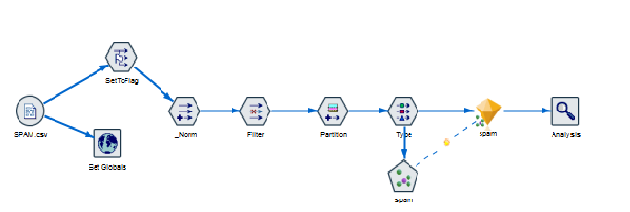
\includegraphics[scale=0.6]{KNN_SPSS.png}
\end{center}
\caption{Analiza modela k najbližih suseda - SPSS}
\end{figure}
\end{frame}

\subsubsection*{Najbliži susedi KNN - SPSS}
\begin{frame}[fragile]
\frametitle{Najbliži susedi - KNN}
\begin{figure}[ht!]
	\centering
    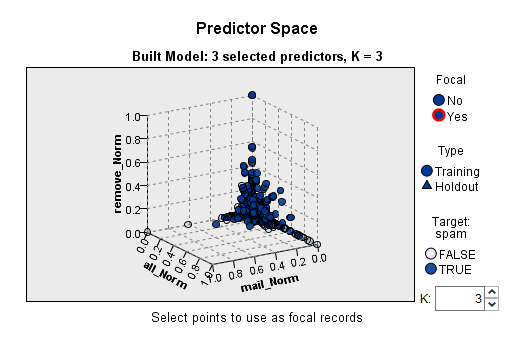
\includegraphics[width=0.5\textwidth]{KNNGrafik.png}
    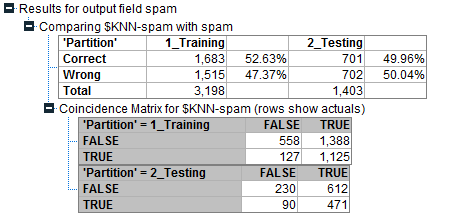
\includegraphics[width=0.4\textwidth]{KNNTabela.png}
    \caption{Grafikom prikazani rezultati KNN-a i Analyze čvora u SPSS-u}
    \label{fig:KNNTabela}
\end{figure}  
\end{frame}

\subsubsection*{Najbliži susedi KNN - Python}
\begin{frame}[fragile]
\frametitle{Najbliži susedi KNN - Python}
\begin{itemize}
\item Trening skup je postavljen na 70\%. 
\item Najbolji rezultati dobijaju se za k = 4
\item Euklidsko rastojanje 
\item Svi susedi imaju podjednak uticaj
\end{itemize}
\end{frame}

\subsubsection*{Najbliži susedi KNN - Python}
\begin{frame}[fragile]
\frametitle{Najbliži susedi KNN - Python}

\begin{lstlisting}
weights_values = ['uniform', 'distance']
#uniform
#Matrica konfuzije
[[793  44]
 [209 335]]

Preciznost 0.8167994207096307
#Izvestaj klasifikacije:
              precision    recall  f1-score   support

     netacno       0.79      0.95      0.86       837
       tacno       0.88      0.62      0.73       544

\end{lstlisting} 

\end{frame}

\subsubsection*{Najbliži susedi KNN - Python}
\begin{frame}[fragile]
\frametitle{Najbliži susedi - KNN}

\begin{lstlisting}

#distance
#Matrica konfuzije
[[770  67]
 [163 381]]

Preciznost 0.833454018826937
#Izvestaj klasifikacije:
              precision    recall  f1-score   support

     netacno       0.83      0.92      0.87       837
       tacno       0.85      0.70      0.77       544

\end{lstlisting} 

\end{frame}

\subsection{Neuronske mreže}
\subsubsection*{Neuronske mreže - SPSS}
\begin{frame}[fragile]
\frametitle{Neuronske mreže - SPSS}

\begin{figure}
\begin{center}
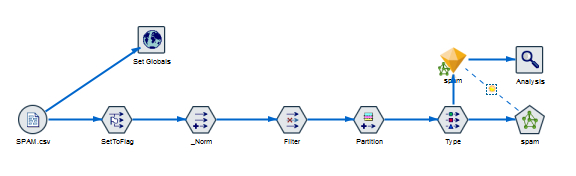
\includegraphics[width=0.8\textwidth]{Neuronske_SPSS.png}
\caption{Model Neuronske mreže u SPSS-u}
\end{center}
\end{figure}
\end{frame}

\subsubsection*{Neuronske mreže - SPSS}
\begin{frame}[fragile]
\frametitle{Neuronske mreže - SPSS}
\begin{itemize}
\item Model se generiše pokretanjem čvora \textit{Neural Net}
\item Za cilj je odabrano kreiranje novog višeslojnog modela
\end{itemize}
\begin{figure}[ht!]
    \centering
    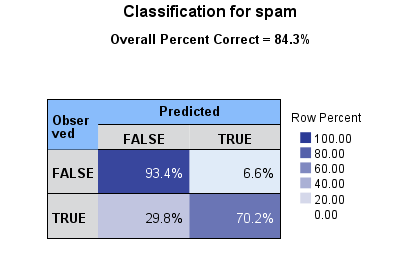
\includegraphics[width=0.5\textwidth]{Neuronske3.png}
    \caption{Matrica konfuzije za neuronske mreže}
    \label{fig:Neuronske3}
\end{figure}
\end{frame}

\subsubsection*{Neuronske mreže - SPSS}
\begin{frame}[fragile]
\frametitle{Neuronske mreže - SPSS}

\begin{figure}[ht!]
    \centering
    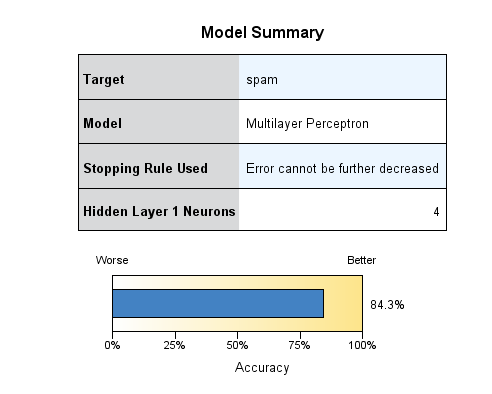
\includegraphics[width=0.5\textwidth]{Neuronske1.png}
    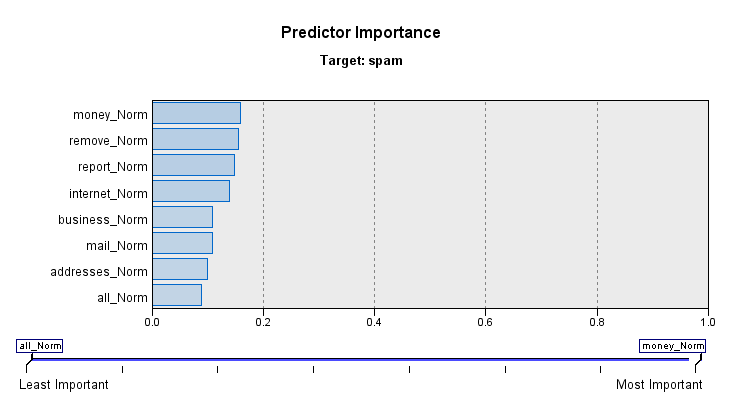
\includegraphics[width=0.5\textwidth]{Neuronske2.png}
    \caption{Neuronska mreža}
    \label{fig:Neuronske1}
\end{figure}
\end{frame}

\subsubsection*{Neuronske mreže - SPSS}
\begin{frame}[fragile]
\frametitle{Neuronske mreže - SPSS}

\begin{figure}[ht!]
    \centering
    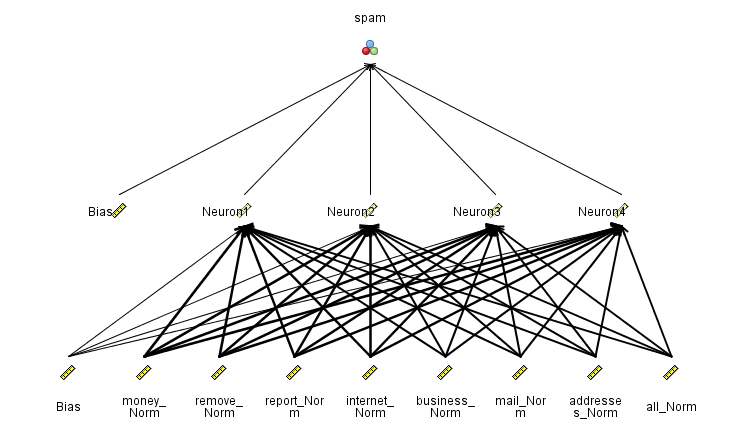
\includegraphics[width=0.75\textwidth]{Neuronske4.png}
    \caption{Neuronska mreža}
    \label{fig:Neuronske1}
\end{figure}
\end{frame}

\subsubsection*{Neuronske mreže - - Python}
\begin{frame}[fragile]
\frametitle{Neuronske mreže - Python}

\begin{lstlisting}
#Izvestaj za test skup:
#Matrica konfuzije
[[786  51]
 [162 382]]
Preciznost 0.8457639391745112
#Izvestaj klasifikacije
              precision    recall  f1-score   support
     netacno       0.83      0.94      0.88       837
       tacno       0.88      0.70      0.78       544

Broj iteracija:  275
Broj slojeva:  4

\end{lstlisting}
\end{frame}


\subsection{Metod potpornih vektora - SVM}
\subsubsection*{Metod potpornih vektora SVM - SPSS}
\begin{frame}[fragile]
\frametitle{Metod potpornih vektora - SVM}
\begin{itemize}
	\item PCA čvor koristimo da bi smanjili skup podataka
	\item SVM čvor pokrećemo i rezultat analiziramo sa Analyse čvorom 
\end{itemize}
\begin{figure}
\begin{center}
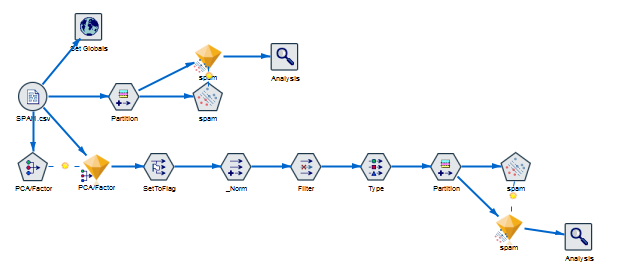
\includegraphics[scale=0.5]{SVM_SPSS.png}
\end{center}
\caption{Metod potpornih vektora - SVM u  SPSS-u}
\end{figure}
\end{frame}


\subsubsection*{Metod potpornih vektora SVM - SPSS}
\begin{frame}[fragile]
\frametitle{Metod potpornih vektora - SVM}

\begin{figure}
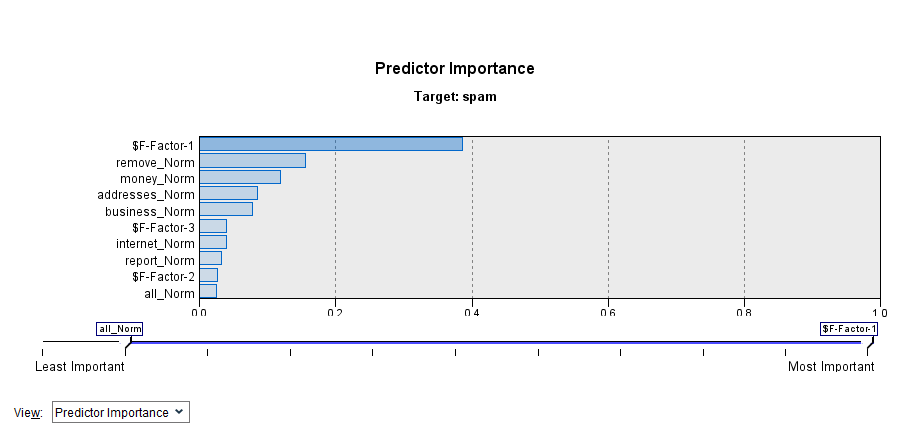
\includegraphics[scale=0.25]{SVMGrafik.png}
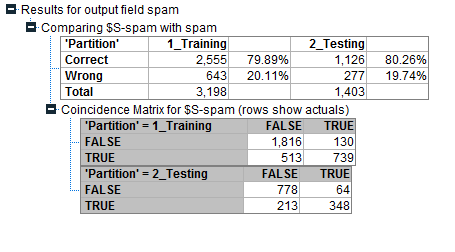
\includegraphics[scale=0.4]{SVMTabela.png}
\caption{Rezultati SVM algoritma dobijeni Analyse čvorom u SPSS-u}
\end{figure}

\end{frame}

\subsection{Gausova klasifikacija}
\subsubsection*{Gausova klasifikacija - Python}
\begin{frame}[fragile]
\frametitle{Gausova klasifikacija}

\begin{lstlisting}
#Matrica konfuzije
[[808  29]
 [306 238]]

Preciznost 0.7574221578566256
#Izvestaj klasifikacije
              precision    recall  f1-score   support

       tacno       0.73      0.97      0.83       837
     netacno       0.89      0.44      0.59       544

\end{lstlisting}
\end{frame}


\section{Zaključak}
\subsection*{Zaključak}
\begin{frame}[fragile]
\frametitle{Zaključak}

\begin{figure}[ht!]
    \centering
    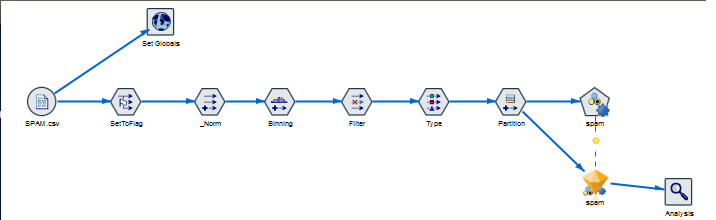
\includegraphics[width=0.7\textwidth]{Poredjenje_SPSS.png}
    \caption{Poređenje svih algoritama u SPSS-u pomoću čvora \textbf{Auto Classifier}}
    \label{fig:Poredjenje_SPSS}
\end{figure}
\end{frame}

\subsection*{Zaključak}
\begin{frame}[fragile]
\frametitle{Zaključak}
\begin{figure}[ht!]
    \centering
    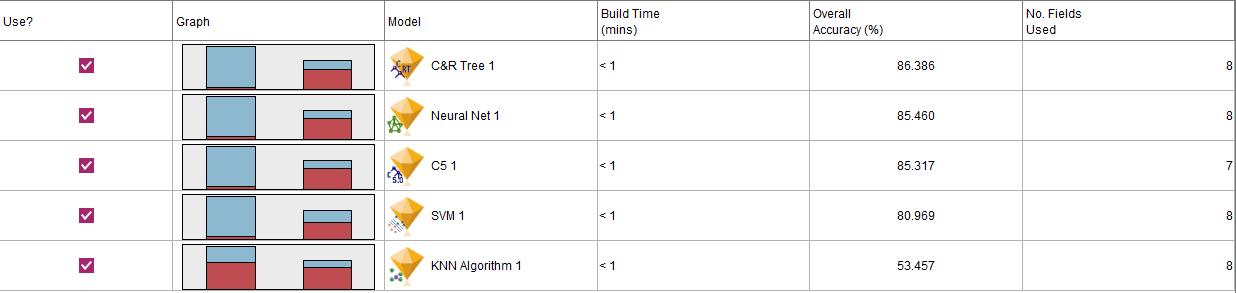
\includegraphics[width=1\textwidth]{Poredjenje.png}
    \caption{Rezultat Analyze čvora nad čvorom koji poredi sve metode}
    \label{fig:PoredjenjeTabela}
\end{figure}
\end{frame}

\section{}
\begin{frame}{}
 \begin{center}
 	\textbf {Hvala na pažnji!}
 \end{center}
\end{frame}

\end{document}